\lecture{13}{22. April 2025}{Varmetransmission}

\section{Mekanismer for varmetransmission}

\subsection{Definition af varmetransmission}
For at kunne arbejde med varmetransmission er det vigtigt at have nogle grundlæggende begreber på plads

\begin{definition}[Varmetransmission]
  Varmetransmission er en løbende, irreversibel varmetransport mellem legemer af forskellig temperatur.
\end{definition}

Overordnet kan dette inddeles i tre forskellige transmissionsmåder:
\begin{itemize}
  \item \textbf{Varmeledning}: Varmeledning er overførsel af energi ved tilfældige stød mellem atomare partikler uden at der sker stoftransport
  \item \textbf{Konvektion}: Ved konvektion overføres energi gennem bevægelsen af en fluid mellem et varmt og et koldt legeme, alså en stoftransport af væske eller gas
  \item \textbf{Varmestråling}: Ved varmestråling overføres energi i form af elektromagnetisk stråling mellem flader
\end{itemize}

\subsection{Sammensat varmeoverføring}
For at illustrer kompleksiteten af mange varmeoverførlser betragtes på \textbf{\autoref{fig:f13_1}} en tagkonstruktion. 
\begin{figure} [ht]
  \centering
  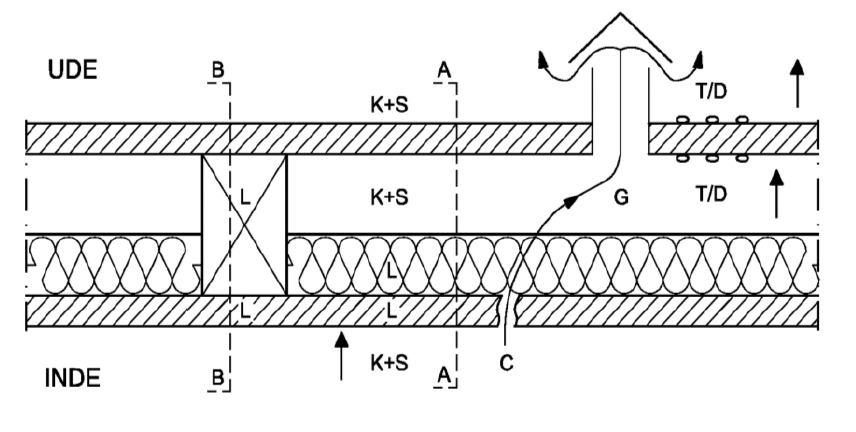
\includegraphics[width=0.5\linewidth]{./figures/f13_1.png}
  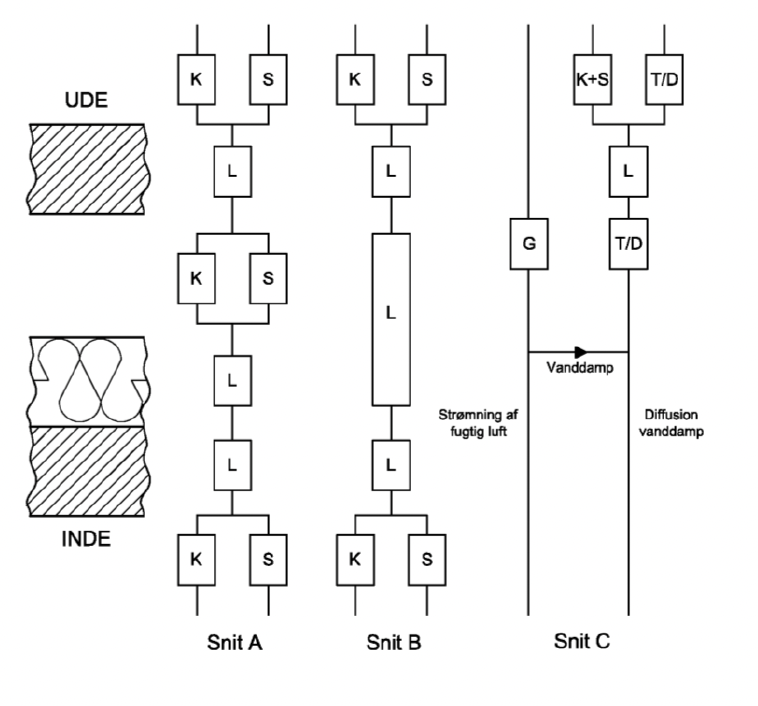
\includegraphics[width=0.4\linewidth]{./figures/f13_1_1.png}
  \caption{Snit gennem en tagkonstruktion}
  \label{fig:f13_1}
\end{figure}
På snittet er brugt følgende forkortelser:
\begin{align*}
  \text{L}&: \text{Ledning} & \text{G}&: \text{Strømning} \\
  \text{S}&: \text{Stråling} & \text{D}&: \text{Fordampning} \\
  \text{K}&: \text{Konvektion} & \text{T}&: \text{Fortætning}
.\end{align*}

\subsubsection{Isolans}
På højresiden af \textbf{\autoref{fig:f13_1}} er de enkelte snit i tagkonstruktionen illustreret med et blokdiagram for at give et bedre overblik. Varmetransmissionsvejene kan illustreres med modstande, eller isolanser, der indikeres med symbolet $R \left[ \unit{m^2 K / W} \right]$ Begrebet er analogt til modstande i el-læren. Her yder modstandene blot en modstand mod strøm af varme. Dette er vist på \textbf{\autoref{fig:f13_2}}
\begin{figure} [ht]
  \centering
  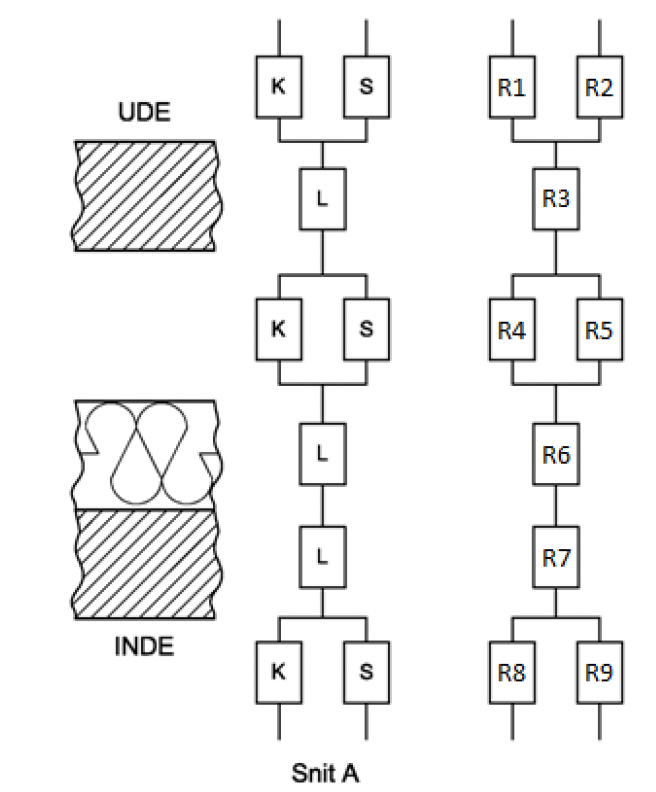
\includegraphics[width=0.5\linewidth]{./figures/f13_2.png}
  \caption{Isolanser fra snit A som modstande}
  \label{fig:f13_2}
\end{figure}

I en bygningskonstruktion er isolanserne for to på hinanden følgende lag seriekoblede. I dette tilfælde, se \textbf{\autoref{fig:f13_2}}, er isolans $R_6$ og $R_7$ koblet i serie og den samlede isolans af de to $R_{6-7}$ findes som:
\[ 
R_{6-7} = R_6 + R_7
.\]
Hvis de to isolanser i stedet var parallelkoblede, sådan som f.eks. isolanserne for konvektion og stråling ved luftlag (f.eks. isolans $R_4$ og $R_5$ i \textbf{\autoref{fig:f13_2}}), findes den samlede isolans $R_{4-5}$ som:
\begin{align*}
  \frac{1}{R_{4-5}} &= \frac{1}{R_4} + \frac{1}{R_5} \\
  \implies R_{4-5} &= \frac{1}{\frac{1}{R_4} + \frac{1}{R_5}}
.\end{align*}
Idet isolanser enten er serie- eller parallelkoblede kan isolansen af enhver konstruktion findes vha. disse to formler.

\subsubsection{Overgangsisolanser}
På samme måde som der er isolanser for de enkelte lag, er der også en isolans mellem den fri luft og overfladerne af konstruktionen. Overgangsisolanserne, $R_{se}$ og $R_{si}$, er sammensat af konvektion og stråling og kan beregnes ud fra formler for konvektion og stråling. De samlede overgangsisolanser findes da til:
\begin{align*}
  R_{se} &= \frac{1}{\frac{1}{R_1} + \frac{1}{R_2}} \\
  R_{si} &= \frac{1}{\frac{1}{R_8} + \frac{1}{R_9}}
.\end{align*}
Typisk vil disse være så små at en standardværdi kan benyttes uden stor fejlmargin. På \textbf{\autoref{fig:f13_3}} er en række standardværdier for overgangsisolanser vist.

\begin{figure} [ht]
  \centering
  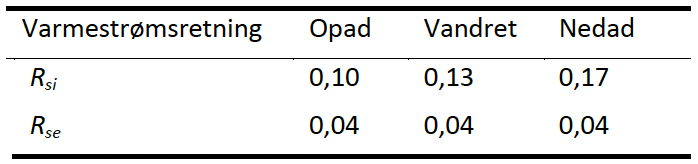
\includegraphics[width=0.5\linewidth]{./figures/f13_3.png}
  \caption{Standardværdier for indvendig og udvendig overgangsisolans i $\unit{m^2 K / W}$}
  \label{fig:f13_3}
\end{figure}

\subsubsection{Varmeoverføringskoefficient}
I visse sammenhænge benyttes også varmeoverføringskoefficienten $h \left[ \unit{\frac{W}{m^2 K}} \right]$ i stedet for isolansen. Varmeoverføringskoefficienten er blot isolansens reciprokke, som:
\[ 
h = \frac{1}{R}
.\]
Dette gælder for hvert enkelt lag af isolanserne. Varmeoverføringskoefficienterne bruges kun om de enkelte lag i konstruktionen og ikke om hele konstruktionen, hvor varmetransmissionskoefficienten $U$ benyttes. 

Der findes også en varmeovergangskoefficient på samme måde som der findes en overgangsisolans.


\subsubsection{Varmetransmissionskoefficient}
Varmetransmissionen, eller varmetabet, gennem en arealenhed af en konstruktion pr. grad \unit{K} temperaturforskel over konstruktionen kaldes varmetransmissionskoefficienten eller $U$-værdien. U-værdien er den reciprokke værdi af konstruktionens totale isolans, inklusive overgangsisolanser:
\[ 
U = \frac{1}{R_{\mathrm{total}}}
.\]
En lille varmetransmissionskoefficient udtrykker en godt isolerende væk. Ydervægge og tage i nybyggeri har typisk $U = \num{0,15} -- \qty{0,3}{\frac{W}{m^2 K}}$. 


\section{Endimensional varmeledning gennem homogene lag}
På \textbf{\autoref{fig:f13_4}} angiver $\Phi$ varmestrømmen gennem et fladeareal $A$, mens størrelsen $q$ angiver varmestrømstætheden, der er varmestrømmen pr. enhedsareal af fladen. 
\begin{figure} [ht]
  \centering
  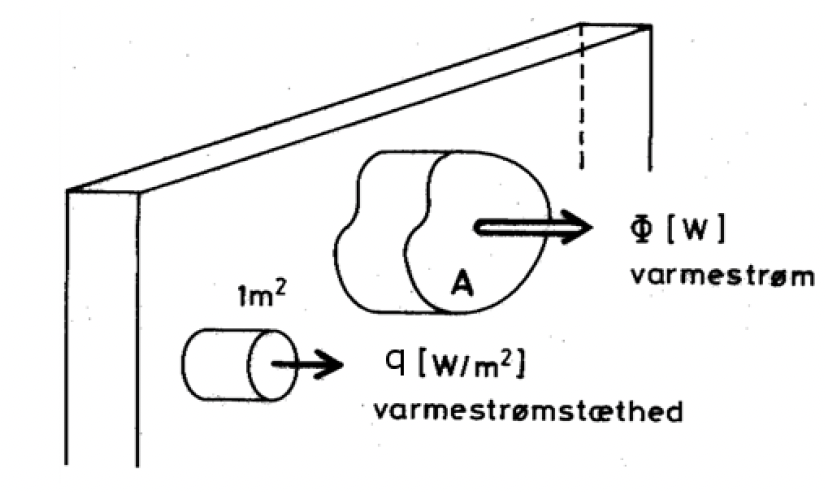
\includegraphics[width=0.5\linewidth]{./figures/f13_4.png}
  \caption{Definition af varmestrøm og varmestrømstæthed}
  \label{fig:f13_4}
\end{figure}

Mellem de to størrelser gælder:
\[ 
\Phi = q_m \cdot A
.\]
En generel to- eller tredimensional betragtning af $q$ sker ud fra Fouriers lov kombineret med en kontinuitetsberegning for varmen. For endimensional strømning parallelt med $x$-aksen lyder Fouriers lov:
\[ 
q = -\lambda \frac{\mathrm{d}T}{\mathrm{d}x} 
.\]
Varmestrømstætheden, $q$, i den givne retning $x$ er ifølge Fouriers lov proportional med temperaturens fald pr. længdeenhed i samme retning. Proportionalitetsfaktoren $\lambda$ afhænger af det betragtede materiales termiske egenskaber.

I en homogen væk med ensartet tykkelse og stor udtrækning forløber varmestrømmen endimensionalt gennem væggen. Dette er vist på \textbf{\autoref{fig:f13_5}}
\begin{figure} [ht]
  \centering
  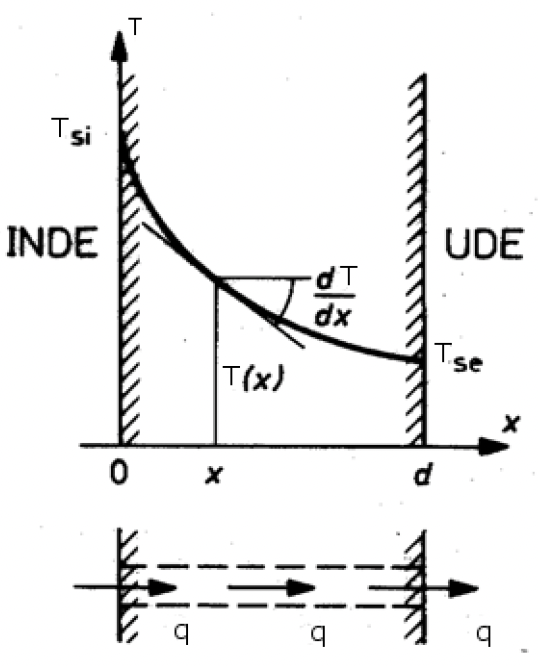
\includegraphics[width=0.5\linewidth]{./figures/f13_5.png}
  \caption{Temperaturgradient ved endimensional strømning gennem homogen væg}
  \label{fig:f13_5}
\end{figure}

Vi kan omskrive Fouriers lov fra før til:
\[ 
\frac{\mathrm{d}T}{\mathrm{d}x} = - \frac{q}{\lambda}
\]
hvor $q$ er konstant (uafhængig af $x$). Integration af dette giver:
\[ 
T = - \frac{q}{\lambda}x + T_{si}
\]
idet $T = T_{si}$ er indsat som randbetingelsen for $x=0$. Temperaturen varierer altså retlinet gennem væggen. Den anden randbetingelse $T=T_{se}$ for $x=d$ kan nu indsættes som:
\[ 
T_{se} = - \frac{q}{\lambda} d + T_{si}
.\]
Hermes kan varmestrømstætheden isoleres som:
\[ 
q = \lambda \frac{T_{si} - T_{se}}{d} = \frac{T_{si} - T_{se}}{R_m}
\]
hvor $R_m$ er den homogene vægs isolans:
\begin{equation}\label{eq:isolans}
  R_m = \frac{d}{\lambda}
\end{equation}
I formlen ovenfor er $T_{si}$ og $T_{se}$ overfladetemperaturer og ikke lufttemperaturer. 

Ved at benytte varmeovergangskoefficienterne $h$ kan effektoverførslerne skrives på formen:
\begin{align*}
  q &= h_i \left( T_i - T_{si} \right) = \frac{T_i - T_{si}}{R_{si}} \\
  q &= h_e \left( T_{se} - T_e \right) = \frac{T_{se} - T_e}{R_{se}}
.\end{align*}
Ved at kombinere dette med udtrykket for effektoverførslen fra før fås:
\begin{align*}
  T_i - T_e &= q \cdot \left( R_m + R_{si} + R_{se} \right) \\
  \implies q &= \frac{T_i - T_e}{R_{si} + R_m + R_{se}}
.\end{align*}
Denne formel kan løses for hvert lag i en samlet konstruktion hvorved den samlede varmestrøm gennem hele væggen kan findes som:
\[ 
\Phi = q \cdot A = U \cdot A \cdot \left( T_i - T_e \right)
.\]

Isolansen at et luftlag kan ikke bestemmes ved den simple formel i \textbf{\autoref{eq:isolans}} som gælder for faste materialer. Dette skyldes, at luftens stråling og eventuelle konvektion kan være langt væsentligere end varmeledningen. 

\section{Endimensional varmeledning gennem inhomogene lag}
Inhomogene lag er lag, der består af forskellige materialer, når et tværsnit vinkelret på varmestrømmens retning betragtes. Beregning af varmeledning igennem disse lag kan tilnærmelsesvist foretages på samme måde som gennem homogene lag, når forskellen mellem varmeledningsevnerne for de forskellige materialer ikke er for stor (højst ca. en faktor 4 forskel i $\lambda$). For at forenkle beregningerne ved inhomogene lag benyttes et vægtet gennemsnit af materialernes varmeledningsevne ud fra deres udbredelse målt vinkelret på varmestrømmens retning.

\section{Konvektion}
Konvektion er medføringen af varme ved strømningen af en fluid. I alle fluider, der bevæger sig, finder der samtidig varmeledning sted i selve fluidet. Denne varmeledning er som regel så lille at den også blot betragtes som en del af ``konvektion''.

Typisk finder konvektiv varmeoverføring sted i følgende tilfælde:
\begin{enumerate}
  \item Ved luftens strømning hen over en plan flade. Som f.eks. vind langs en ydervæg. Varmen overføres fra selve  overfladen til ``et sted'', der er tilstrækkeligt langt ude i den omgivende luft til at være upåvirket af fladen.
  \item Ved strømning indvendigt i rør (som regel væske) eller kanaler (som regel luft). Den konvektive varmetransport overfører her varmen mellem kanal/rør-væggen og fluidet. 
  \item Ved strømning mellem to parallelle flader, der adskilles af et luftlag eller evt. en væske. Her vil der dannes en hvirvlende strøm mellem de to overflader.
  \item Et særligt tilfælde af 1 er et fluids strømning hen over ydersiden af et rør eller en kanal. Dette finder man typisk i varmtvandsbeholdere. 
\end{enumerate}

Der skelnes typisk mellem to former for konvektion, hvor styrken til at overføre varme igen afhænger af hvilken af de to strømningstyper, der er gældende. De to former for konvektion er:
\begin{itemize}
  \item \textbf{Tvungen konvektion}, hvor fluidets bevægelse skyldes udefrakommende kræfter som f.eks. en ventilator, en pumpe eller vinden. 
  \item \textbf{Naturlig konvektion}, hvor fluidets bevægelse skyldes temperaturforskelle, der forårsager forskelle i massefylde. 
\end{itemize}

Generalt inddeles konvektion også i hhv. laminar strømning og turbulent strømning.

\subsection{Laminar strømning}
Helt inde ved den bestrøgede overflade står fluidet stille. Herover flyder fluidets molekyler roligt som molekylelag, hvis bevægelser er parallelle med den bestrøgede overflade. Molekylelagenes hastighed udvikler sig i et krumt forløb med afstanden fra overfladen, indtil hastigheden et stykke ude når den fri strømningshastighed. 

Hastighedsprofilet udvikles fra væggen som en såkaldt Blasius-profil, hvis eksakte løsning ikke kan skrives med en simpel formel. Området fra den bestrøgede overflade indtil fluidet når den fri strømningshastighed kaldes grænselaget. Strømningsprofilen i grænselaget er uafhængigt af den bestrøgede overflades karakter. Temperaturen følger en lignende profil, dog af og til med en anden tykkelse.

Da strømningen er rolig og overvejende parallel med overfladen, er den konvektive varmeoverførsel kun lidt større end ren varmeledning i fluidet mellem overfladen og det fri strømningsfelt.

\subsection{Turbulent strømning}
Ved store hastigheder bliver strømningen urolig. Her finder der talrige små fluktuationer sted, som går på tværs af den bestrøgne overflade. I ethvert punkt og i alle retninger ændres hastigheden løbende. Hastigheden er stadig nul helt inde ved den bestrøgne overflade, men den udvikles hurtigt væk fra overfladen. Helt inde ved overfladen findes dog et laminart sublag, hvor hastighed og temperatur udvikles lineært. Udenfor det laminare sublag udvikles hastigheden tilnærmelsesvist med logaritmen til afstanden til væggen.

Tilsvarende har temperaturprofilet en hurtig udvikling væk fra overfladen, hvor fluidet har overfladens temperatur ud til den afstand, hvor det fri strømningsfelts temperatur opnås. Ved turbulent strømning spiller overfladekarakteren ind i langt højere grad end for laminar strømning.

\subsection{Beregningsmetode}
Uanset konvektionsform, strømningstype og anvendelse ønsker man at nå frem til at kunne beskrive varmeoverføring med den simple ligning:
\[ 
\Phi = A \cdot h_k \cdot \Delta T
.\]
I stedet for den konvektive varmeovergangskoefficient $h_k$ kan den kollektive overgangsisolans $R_k$ benyttes:
\[ 
R_k = \frac{1}{h_k}
.\]
Desværre kan den konvektive varmeovergangskoeffienct ofte ikke bestemmes teoretisk med stor nøjagtighed. 
